\chapter{Future nEDM Measurement at TRIUMF\label{chap:nedm}}

Finding a non-zero neutron electric dipole moment~(nEDM) is directly
linked to the extra sources of $CP$ violation beyond the Standard
Model.  The next generation of nEDM experiments aim to measure $d_n$
with proposed precision
$\delta d_n\lesssim
10^{-27}~e\cdot$cm~\cite{serebrov2014new,serebrov2011supersource,Kirch_talk,baker2011search,altarev2012next,golub1994neutron,ito2007plans,picker2017minuscule}.
The TUCAN~(TRIUMF UltraCold Advanced Neutron source) collaboration
proposes a world-leading experiment to measure the nEDM, improving the
precision by a factor of thirty compared to the present world’s best
experimental result. The current nEDM experiments suffer from low UCN
statistics and a key goal is to build the strongest UCN source in the
world. To achieve this goal, extensive studies of the current vertical
UCN source have been conducted~(See Chapters~\ref{chap:UCNattriumf}
and ~\ref{chap:UCNresult}).



\section{TRIUMF nEDM Components~\label{sec:triumfnedm}}
In 2016, the vertical UCN source from RCNP in Japan was shipped to
TRIUMF for the research towards the development of the new upgraded
UCN source.  The details of the current UCN facility at TRIUMF is
presented in Chapter~\ref{chap:UCNattriumf}. The result of the first
set of UCN experiments with the vertical UCN source is available in
Chapter~\ref{chap:UCNresult}.



The future nEDM experiment at TRIUMF will use a room-temperature nEDM
apparatus, connected to an upgraded cryogenic UCN
source~Fig~\ref{fig:triumfEDM}. A proton beam at 480~MeV and 40~$\mu$A
impinges on a tungsten spallation target liberating neutrons. Over the
target, a room-temperature neutron moderator/reflector system composed
of Pb, graphite, and D$_2$O thermalizes the neutrons. Liquid
deuterium~(LD$_2$) at 20~K creates a large flux of cold neutrons~(CN)
in a bottle containing superfluid $^4$He below 1~K. In the superfluid
helium, the CN excite phonon and roton transitions, losing virtually
all their kinetic energy to become UCN. Once a sufficient density of
UCN is built up, the proton beam is turned off, and a cryogenic UCN
valve opens. The UCN are transported out of the source by specular
reflection on the surfaces of the UCN guides. A superconducting
magnet~(SCM) accelerates polarized UCN through barrier foils to a
vacuum volume at room temperature. The UCN are then transported to the
nEDM experiment by additional guides.
%The cyclotron at TRIUMF produces a~$\sim$~500~MeV proton beam. Protons
%are guided to the spallation target using a variety of
%magnets. Spallation neutrons are moderated and converted to UCN in a
%superfluid He-II volume, which diffuse through UCN guides to the nEDM
%measurement cell.



\begin{figure}[h!]
  \centering
  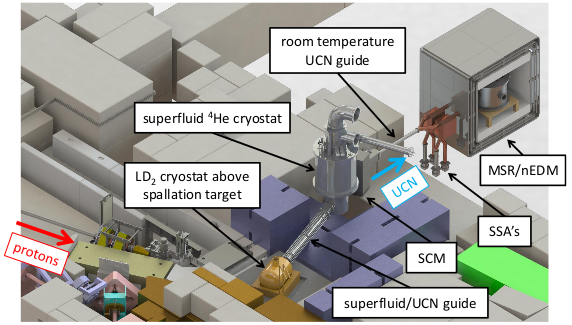
\includegraphics[width=1.0\textwidth]{edmtriumf.png}
  \caption[Conceptual design of TUCAN's future nEDM
  facility]{Conceptual design of the proposed UCN source and nEDM
    experiment. Protons strike a tungsten spallation target. Neutrons
    are moderated in the LD$_2$ cryostat and become UCN in a
    superfluid $^4$He bottle, which is cooled by another cryostat
    located farther downstream. UCN pass through guides and the
    superconducting magnet~(SCM) to reach the nEDM experiment located
    within a magnetically shielded room~(MSR). Simultaneous spin
    analyzers~(SSA’s) detect the UCN at the end of each nEDM
    experimental cycle.  }
  \label{fig:triumfEDM}
\end{figure}

%A schematic overview of the proposed UCN source upgrades, and the nEDM
%experiment is presented in Fig.~\ref{fig:triumfEDM}.
A brief description of the main components of the future nEDM apparatus
at TRIUMF is presented below.

\subsection{New UCN Source\label{sec:newUCNsource}}


The future nEDM experiment at TRIUMF will use an upgraded UCN source,
which has quite some differences with the vertical UCN source
described in Chapter~\ref{chap:UCNattriumf}. A conceptual design of
the next generation UCN source is shown in
Fig.~\ref{fig:newUCNsource_2}. The upgraded source is referred to as
``the new horizontal source'', because the UCN exit in a
near-horizontal direction. When UCN exit the He-II into vacuum, they
gain a kinetic energy equivalent to the neutron optical potential of
18.5~neV. This corresponds to a height in Earth’s gravity field of
18.1~cm. Therefore near-horizontal extraction of UCN is a reasonable
development for He-II sources.


The moderators and the He-II cryostat are surrounded by shielding blocks
made of steel. Additionally, neutron absorbers made of borated
polyethylene~(PE) line the moderators and the UCN guide to reduce
activation of the steel blocks by thermal neutrons. Including a 10~cm
of steel shielding and 5~cm of borated polyethylene, significantly
reduces the activation of the cryostat in cases with large shielding
penetrations.

The heavy-water moderator at room temperature is a thermal
pre-moderator for fast neutrons, reducing the required amount of cold
moderator and the heat load on the cold moderator and UCN
converter. Additionally, it is placed around the cold moderator to
reflect thermal neutrons back into it. Additional graphite blocks
serve as reflectors. The spallation target is covered with a layer of
lead, which has a low neutron-absorption cross section and shields the
cold moderator and converter from $\gamma$ radiation.

The purpose of the cold moderator system is to produce the maximum
number of 1~meV neutrons, with the minimum number of neutron captures
in the material. Minimizing the neutron captures is important to
prevent production of gamma rays which would heat the He-II in the UCN
production volume, as well as to minimize neutron loss (for this
reason, deuterated materials are preferable). Higher energy $>$~1~meV
neutrons can also be used, since multiphonon excitations in the
superfluid can potentially produce UCN as discussed in
Section~\ref{sec:UCN_production}~\cite{Schmidt2009,
  Korobkina2002}. The new UCN source uses an LD$_2$ cryostat to
produce cold neutrons during the experiment, as opposed to the solid
D$_2$O in the vertical source. LD$_2$ increases the UCN production by
a factor of 2-3, and reduces the heat load and the uncertainty in the
UCN source performance.



The UCN production and detection of the new source are estimated in
details based on an Monte Carlo N-Particle~(MCNP) model of the source,
an analytical model of UCN production based on
Ref.~\cite{Korobkina2002}, and UCN transport simulations based on
Ref.~\cite{schreyer2017pentrack} including losses on walls and within
the He-II and the vapour pressure above it.  The simulations indicate
that when driven by a 40~$\mu$A proton beam, the source will produce
$2\times 10^7$~UCN/s, with beam heating to the He-II $<~10$~W, a
design goal for our refrigerator. At the end of target irradiation,
$3.4\times 10^8$~UCN would be in the source prior to opening the
room-temperature valve~(not shown in Fig.~\ref{fig:newUCNsource_2}) to
the nEDM experiment.  The simulations also include transport into the
nEDM experiment. A total of $6.5 \times 10^6$~UCN would be loaded into
the EDM measurement cells prior to initiating the Ramsey cycle. Using
reasonable values for lifetimes and spin-coherence times of the
UCN~(storage lifetime of 120~s or higher, and $T_1 = 1000$~a and
$T_2 = 500$~s~\cite{cdr2018}), this corresponds to a statistical
determination of the nEDM of
$\sigma(d_n) = 3\times 10^{-25}$~e$\cdot$cm per cycle. With reasonable
assumptions for the running time available per day, a statistical
determination of $\sigma(d_n) = 10^{-27}$~e$\cdot$cm would be achieved
in 400 days.

The new UCN source will have several key improvements. Foremost of these
is improved heat exchanger design and improved cooling
efficiency. Also to be improved are the internal neutron guides. We
plan to use an Al-Be alloy bottle presenting a lower heat load to the
He-II. Gamma and beta heating from the Al bottle walls is presently
projected to dominate the heat load to the superfluid. Extraction of
UCN from the source would be improved by the near-horizontal
extraction.

%A room-temperature Al window within a superconducting
%magnet will provide vacuum separation. The Al window will prevent
%contaminants from entering the He-II, while the superconducting magnet
%will accelerate high-field-seeking UCN through the window, resulting
%in highly polarized UCN after extraction.

%\begin{figure}[h!]
%  \centering
%  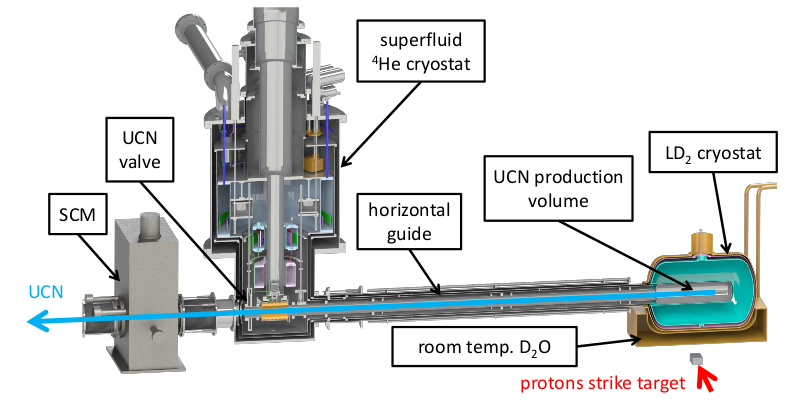
\includegraphics[width=1.0\textwidth]{newUCNsource.png}
%  \caption{The 3D model of the proposed UCN source and the LD$_2$
%    cryostat. Protons strike a tungsten spallation target liberating
%    neutrons, which are moderated in surrounding volumes of graphite
%    (not shown), D$_2$O, and LD$_2$. Neutrons are downscattered in the
%    UCN production volume containing superfluid $^4$He. They are
%    bottled within a horizontal guide up to a UCN valve. When the
%    valve is opened, UCN are transported to room temperature UCN
%    guides.}
%  \label{fig:newUCNsource}
%\end{figure}

\begin{figure}[h!]
  \centering
  \includegraphics[width=1.0\textwidth]{newUCNsource_2.png}
  \caption[Conceptual design of TUCAN's new UCN source]{Conceptual
    design of the next generation UCN source planned for
    TRIUMF. Neutrons are liberated by proton-induced spallation in a
    target located beneath the He-II, and LD$_2$ and D$_2$O
    moderators. Neutrons are reflected and moderated in surrounding
    materials, then enter superfluid $^4$He~(He-II), where they are
    downscattered. Cooling for the superfluid is provided by heat
    exchanger within the He-II cryostat. UCN created in the He-II are
    transported out through the heat exchanger passing through the
    He-II surface into vacuum in a vertical rise, and to the
    experiment which is conducted at room temperature.}
  \label{fig:newUCNsource_2}
\end{figure}

\subsection{UCN Handling and Transport}

Efficient transport of polarized UCN is one of the major requirements
for the nEDM measurement. This efficiency depends mainly on three
parameters: UCN guide wall capacity, surface roughness of the UCN
guides, and UCN polarization. These are described below.

The first parameter is the capacity of the guide walls to contain the
UCN. UCN have a large wavelength compared to the lattice constants in
solid matter~(50 to 130~nm compared to 0.3~nm). Therefore, during a
scattering process, a UCN interacts with hundreds of nuclei. The mean
nuclear potential experienced during the scattering~(Fermi potential)
depends on the material. In order to store UCN, the Fermi potential
must be as high as possible.

The second parameter is the roughness of the surface. Transportation
is more efficient if the roughness is low because, the probability of
specular reflection is increased. Ideally, the roughness should be
lower than the UCN wavelength of~$\sim 40$~nm but, in practice this is
challenging to achieve.

The last parameter is related to the polarization. UCN can be
depolarized during a collision due to different processes.
%such as spin incoherent nuclear scattering, paramagnetic scattering or
%large magnetic field gradients.
When selecting materials for UCN components, the mean depolarization
rate per bounce should be as small as possible. In practice this
means, all nonmagnetic coatings for polarized UCN traps.
\begin{figure}[h!]
  \centering
  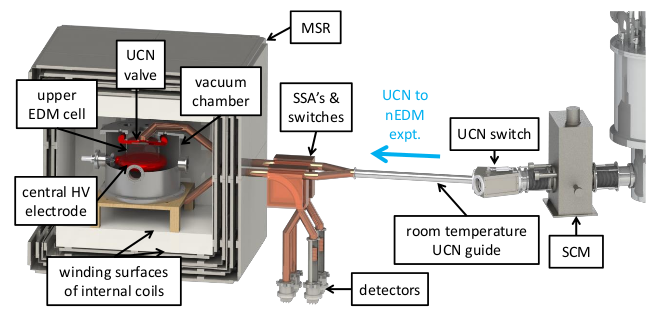
\includegraphics[width=1.0\textwidth]{UCNdelivery.png}
  \caption[3D model of TUCAN's future UCN delivery for the nEDM
  measurement]{A 3D model of the UCN delivery and the future nEDM
    experiment at TRIUMF. UCN exit the source by passing through the
    SCM spin polarizer, and UCN switch and detector system, where they
    then enter the proposed nEDM experiment. UCN are loaded into the
    measurement cells within a MSR/coil system. At the end of the
    measurement cycle, UCN are counted by simultaneous spin
    analyzers~(SSA’s) including detectors. An ambient magnetic
    compensation system, and thermally controlled room, will surround
    the nEDM apparatus~(not shown). For scale, the innermost layer of
    the MSR is a 1.8~m side-length cube.}
  \label{fig:UCNdelivery}
\end{figure}



The main task of the UCN handling parts is to transport a large
phase-space fraction of the UCN most efficiently to achieve the
highest statistical sensitivity in the experiment as possible.

The parts that come in contact with UCN on the way from the UCN source
to the EDM experiment, and the UCN detectors, constitute the neutron
handling hardware: UCN guides, valves, switches and simultaneous spin
analyzer~(SSA) system. Fig.~\ref{fig:UCNdelivery} shows the neutron
handling parts for the future nEDM experiment at TRIUMF.  UCN exiting
the source are polarized by a superconducting magnet~(SCM), and then
enter the nEDM experiment.

Suitable guides and valves have optimized geometries: wall materials
with large Fermi potentials, low upscattering and absorption cross
sections for neutrons, and low roughness and depolarization. The plan is
to use Be for the UCN production volume, and NiMo coatings for most
other surfaces, on glass and Cu substrates, where non-magnetic
polarization preserving guides are required.  

UCN spins will be measured by two separate simultaneous spin analyzer
(SSA) systems (one for each cell). Its configuration allows
simultaneous counting of both UCN spin states, and maximizes the
visibility of the Ramsey fringes and counting efficiency.  The UCN
switches load the UCN into the nEDM experiment, and divert UCN exiting
the experiment into the detectors.  A prototype detector, based on
scintillating lithium glass, and capable of handling the highest rates
of UCN expected with the TRIUMF source has been developed and tested
in the highest rate UCN beam available at
PSI~\cite{jamieson2017characterization}~(See
Chapter~\ref{chap:UCNattriumf}).
%This detector is based on the detector used
%in the PSI UCN experiments~\cite{Ban2009}.



%The cold neutron guides contain liquid helium (shown in purple in
%Fig.~\ref{fig:UCNhandling}) at a temperature of less than 1~K. A cold
%UCN gate valve partitions this volume. Upstream of it, the neutrons
%are stored/accumulated while the proton beam irradiates the
%target. Three aluminum foils constitute the end of the 1~K neutron
%guide section, sitting inside a 3.5~T superconducting magnet, the UCN
%polarizer. A transition region of guides bridges between temperatures
%from 100~K to room temperature, which is the temperature of all
%downstream neutron handling equipment.

%At TRIUMF, the room temperature UCN guide will be split between the
%EDM experiment and the second experiment port via a Y-switch. Towards
%the EDM cell(s), the UCNs pass another UCN switch (aka. rotary valve
%or EDM detector switch) which can either guide neutrons from the
%source to the EDM cell or from the EDM cell to the UCN detectors. Each
%EDM cell itself is closed by a plug (or door valve) to store the
%neutrons during the Ramsey cycle. The vertical section of the UCN
%guides towards the UCN detectors contains spin flippers and spin
%analyzers and the UCN detectors at the bottom.

%To systematically check all possible alignments of electric field,
%magnetic field and neutron spin in the EDM experiment, a spin flipper
%can be added to the UCN guide system after the Y-switch and before it
%is possibly split to serve the two EDM cells. In this way, both
%neutron spin states can be loaded into the experiment. The spin
%analyzer uses a magnetic potential of 60 neV/T to analyze the neutron
%spin direction, deter- mining whether it’s spin is aligned~(low field
%seekers), or anti-aligned~(high field seekers) with the analyzer
%magnetic field.





\subsection{Magnetic Fields in the nEDM Experiment}
To achieve the desired nEDM sensitivity of ~$10^{-27}$~e$\cdot$cm, an
extremely stable and homogeneous $B_0$ magnetic field is required.
The magnetic stability upper limit for TUCAN's nEDM measurement is
1~pT (for hundreds of seconds) and the magnetic homogeneity upper
limit is 1~nT/m.
%beyond which a comagnetometer must be
%used to correct the field to the $\sim$∼10~fT level.
Because of the challenges to achieve this level of magnetic stability,
a $^{199}$Hg co-magnetometer will be used to correct for the $B_0$
field fluctuations. To achieve these specifications, both active and
passive shielding will be utilized to nullify the uncontrolled and
time-varying external fields. The desired internal magnetic field will
be generated by using uniform and shim
coils. Fig.~\ref{fig:magneticscheme} shows the schematic drawing of
the magnetic components of the TUCAN nEDM experiment. Each magnetic
component is explained below.

\begin{figure}[h!]
  \centering
  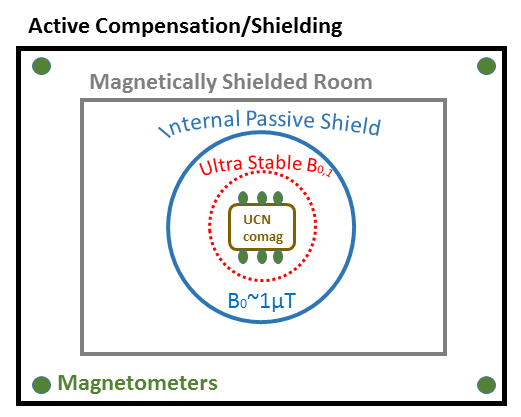
\includegraphics[width=0.7\textwidth]{magneticscheme.png}
  \caption[Schematic of TUCAN's nEDM magnetics components]{Schematic
    drawing for the TUCAN nEDM magnetics. From outside in: The active
    compensation system followed by several layers of magnetically
    shielded room and passive shields nullify the environmental
    magnetic field. The magnetometers inside the active shielding
    monitor the changes in the magnetic field internal to that
    region. The internal coil system~($B_0$ and $B_1$ coils) generate
    the magnetic fields for the Ramsey cycle. The UCN and the
    co-magnetometers are internal to the coils.  }
  \label{fig:magneticscheme}
\end{figure}



\subsubsection{Active Shielding}

The magnetic environment at the location of the planned nEDM
experiment at TRIUMF is dominated by a static field due to the main
cyclotron at TRIUMF which can be as large as 100-400~$\mu$T, with 1 to
100~nT fluctuations due to the other external magnetic sources such as
nearby beam line magnets or the displacement of large magnetic
objects~(e.g., the crane is the Meson Hall).

The TUCAN's plan is to reduce the static field to less than 50~$\mu$T
using dedicated compensation coils and constant-current supplies, with
a readily achievable stability of $10^{-3}$, and to reduce the
remaining static field and fluctuations by up to a factor of 100
through a separate set of compensation coils and current supplies,
using fluxgate magnetometers for magnetic feedback. The fluxgate
sensors will be placed in the region between the compensation coils
and the passive shields as shown in Fig.~\ref{fig:magneticscheme}.  A
prototype active compensation system has been built at the University
of Winnipeg based on Refs.~\cite{beatrice,afach2014dynamic}. The
system employs a set of coils centred around a cylindrical passive
magnetic shield system, using four 3-axis fluxgates for feedback~(see
Fig.~\ref{fig:prototype_active}). Overall, the active shielding system
should be able to reduce the net background magnetic field to the
level of tens of nT over the volume of the nEDM cell.


\begin{figure}[h!]
  \centering
  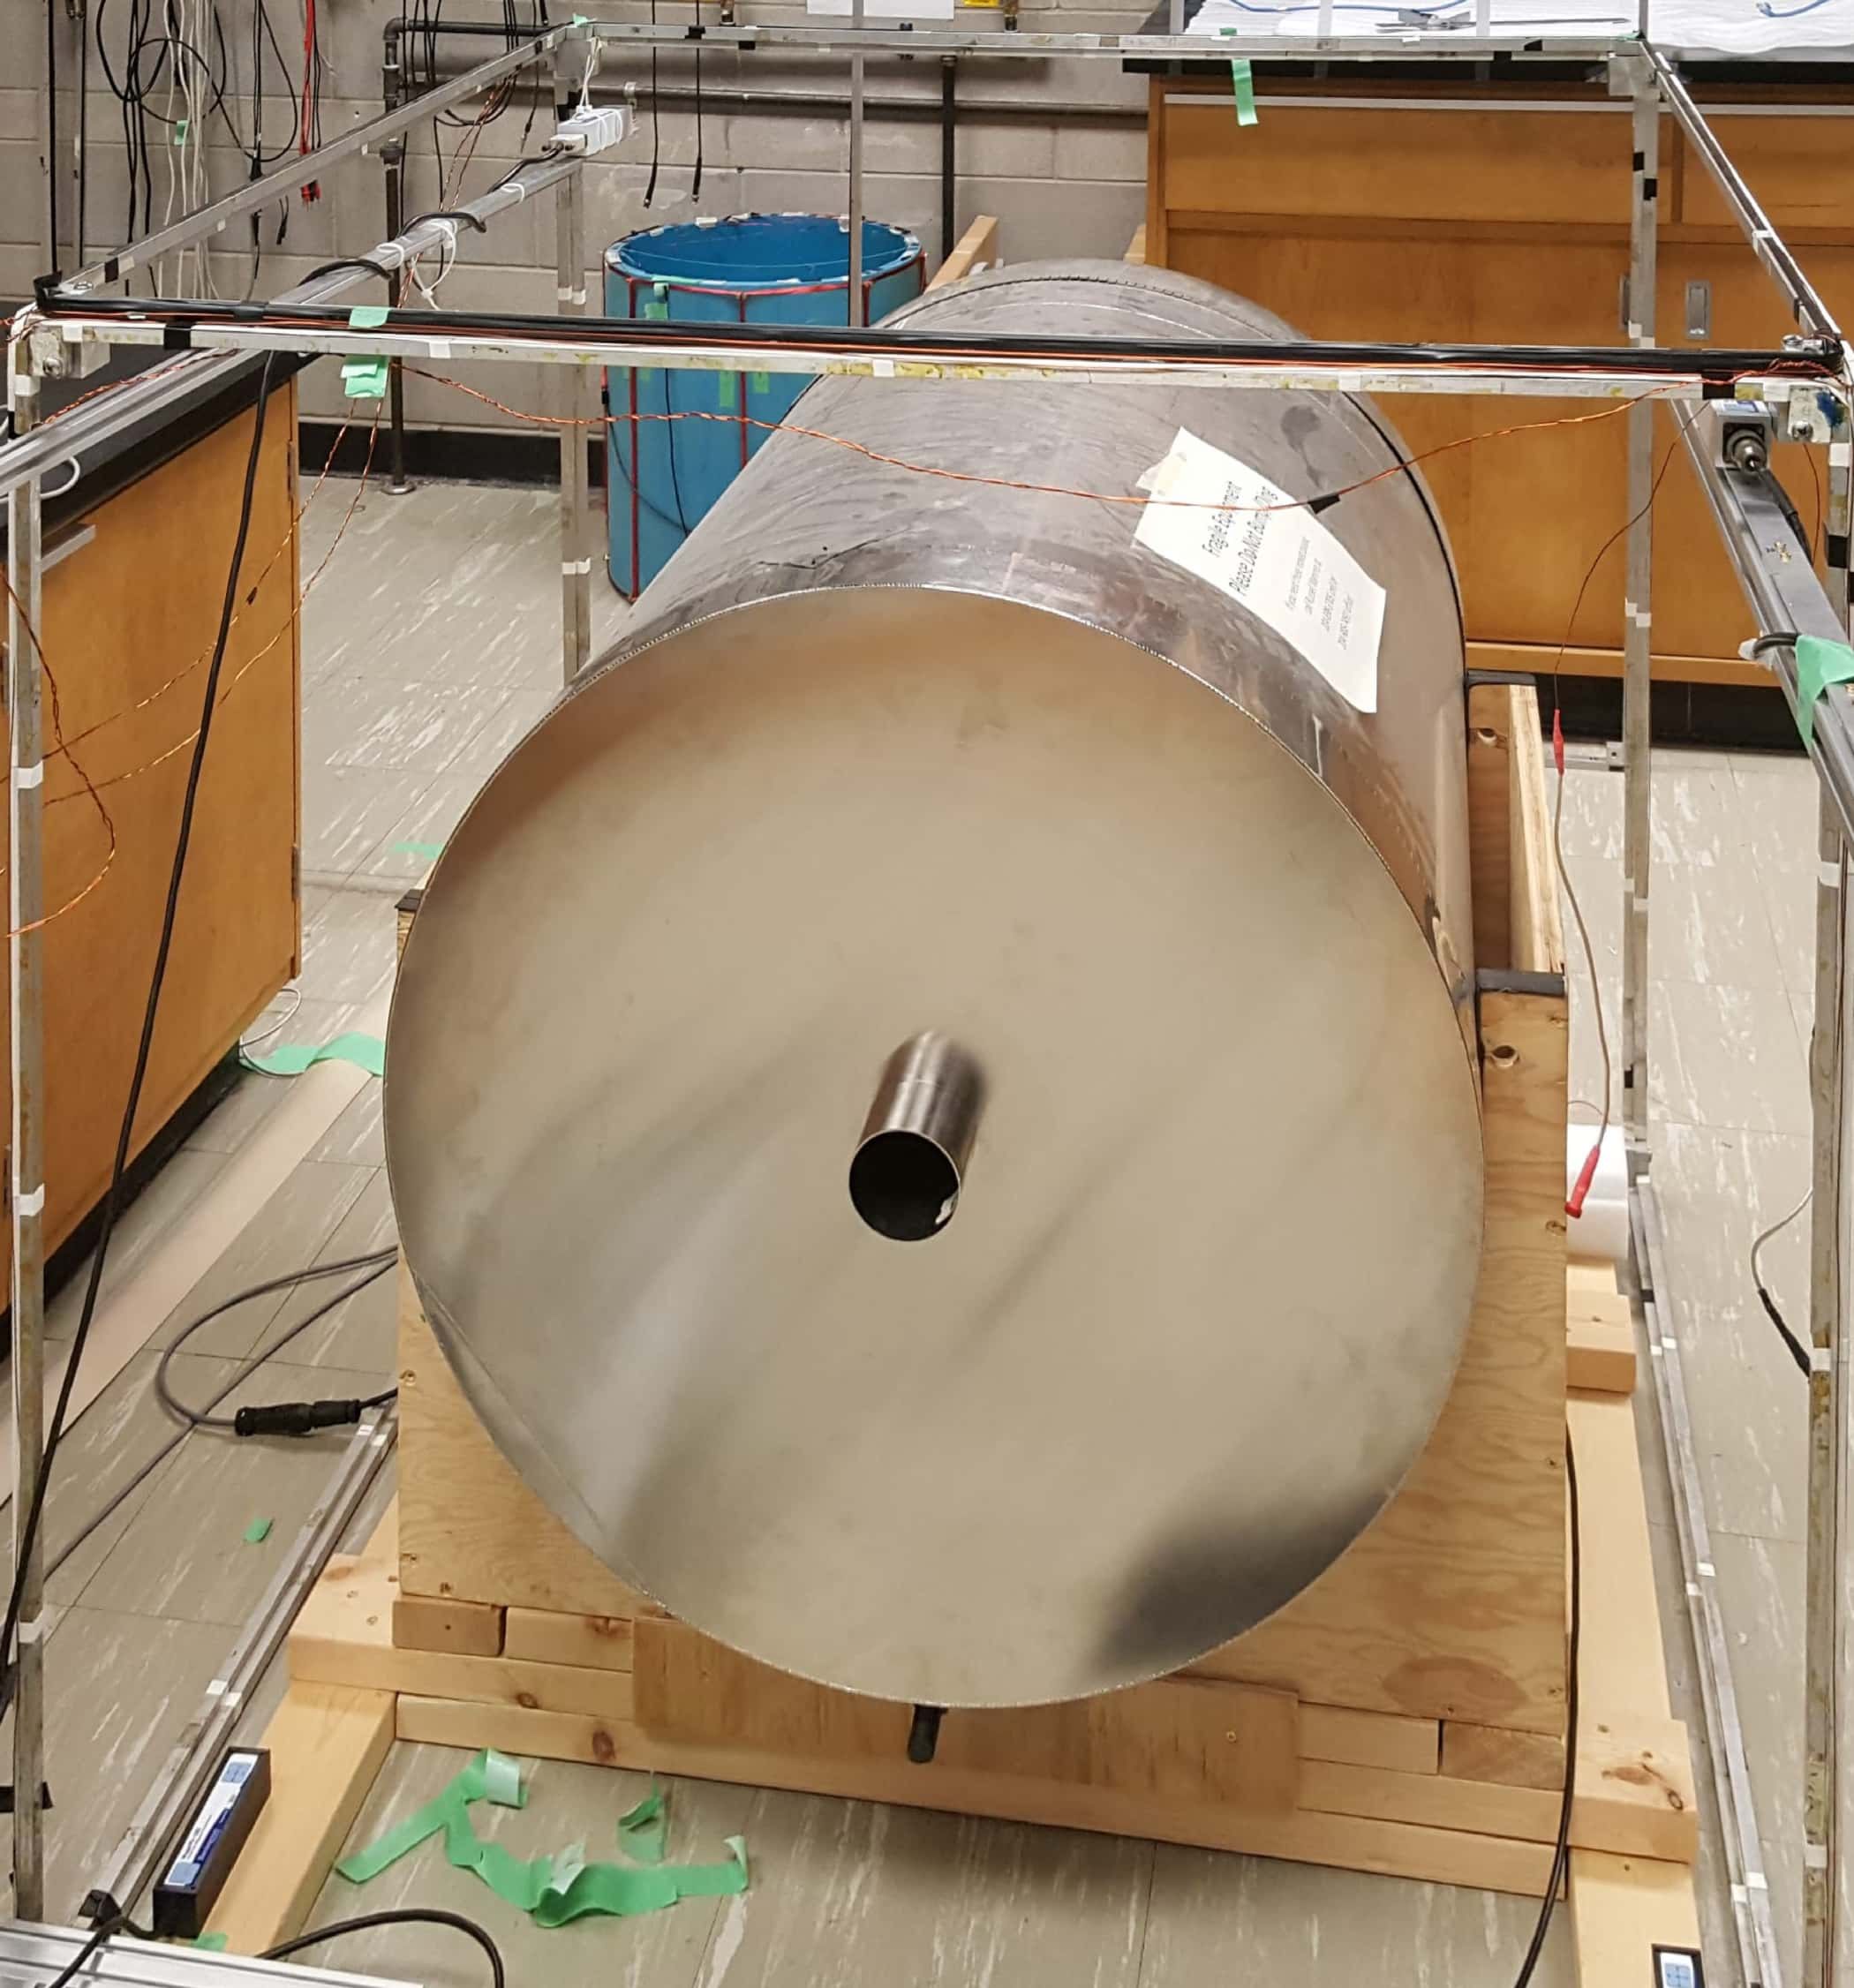
\includegraphics[width=0.7\textwidth]{active_prototype.jpg}
  \caption[TUCAN's prototype active compensation system]{The prototype
    active compensation system at the University of Winnipeg.}
  \label{fig:prototype_active}
\end{figure}

\subsubsection{Passive Shielding}


Passive magnetic shielding system is generally composed of a multi-layer
shield formed from thin shells of material with high magnetic
permeability~(e.g., mu-metal).  The outer layers of the shield are
normally cylindrical~\cite{serebrov2014new,baker2011search} or form
the walls of a magnetically shielded
room~\cite{altarev2014magnetically,altarev2015minimizing}.  The
innermost magnetic shield is normally a specially shaped shield, where
the design of the coil in relation to the shield is carefully taken
into account to achieve adequate
homogeneity~\cite{Baker2006,Kirch_talk,altarev2012next}. Fig.~\ref{fig:prototype_shields}
shows a picture of a prototype passive shield at the University of
Winnipeg, which is in support of the precision magnetic field research
for the future nEDM experiment to be conducted at TRIUMF.  The shield
system is a four-layer mu-metal shield formed from nested
right-circular cylindrical shells with endcaps.  The inner radius of
the innermost shield is 18.44~cm, equal to its half-length. The radii
and half-lengths of the progressively larger outer shields increase
geometrically by a factor of 1.27.  Each cylinder has two endcaps
which possess a 7.5~cm diameter central hole.  A stove-pipe of length
5.5~cm is placed on each hole, was designed to minimize leakage of
external fields into the progressively shielded inner volumes.  The
design is similar to another smaller prototype shield discussed in
Ref.~\cite{martin2015large}.

\begin{figure}[h!]
  \centering
  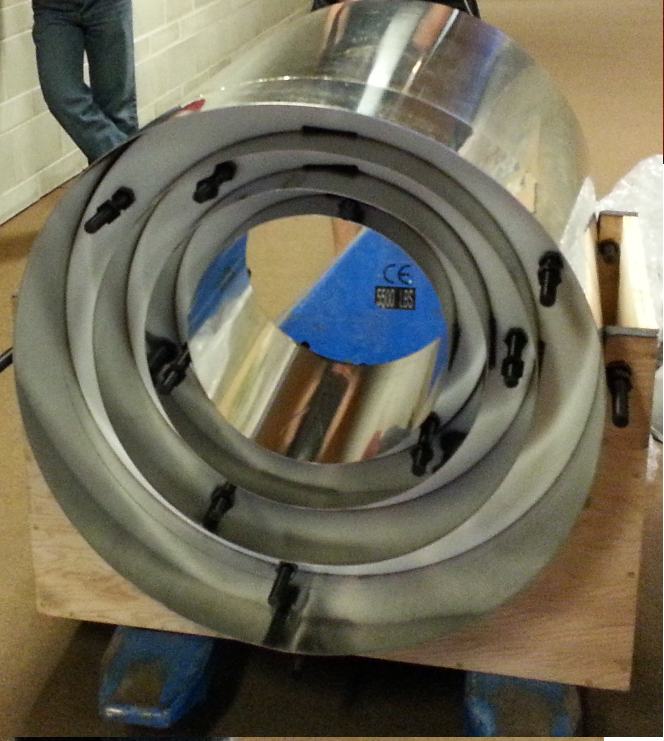
\includegraphics[width=0.6\textwidth]{prototype_shields.png}
  \caption[TUCAN's prototype passive shielding]{Three layers of the
    prototype passive magnetic shield at the University of
    Winnipeg. The 4th layer is not shown in this picture.}
  \label{fig:prototype_shields}
\end{figure}


The TUCAN passive shielding system will reduce the magnetic field to
the pT level.
%It will be a two-stage system: (1) a magnetically
%shielded room~(MSR) with (2) a set of smaller shields that fit inside
%the room and surround the nEDM apparatus.

A magnetically shielded room~(MSR) with quasi-static
shielding factor of $\sim$~100,000 is sufficient to reduce the magnetic
fluctuations to the $\sim$~pT level. A four-layer MSR with an inner
cubic space of side-length 1.8~m and outer side-length 2.8~m produces
this shielding factor, with mu-metal wall thicknesses 2~mm, 6~mm,
4~mm, 4~mm (inner to outer), equally spaced.


The innermost layer of the internal passive shields also may serve as
a return yoke for the magnetic flux generated by the internal coils
for the shield-coupled coil designs. A degaussing~(idealization)
system will be used to stabilize the shields. A combined DC shielding
factor of the order of $10^6$ is expected.


In the case of the shield-coupled coils, if the properties of the
shields changes, the internally measured magnetic field will change.
Changes in the temperature of the magnetic shields gives rise to a
change in the magnetic permeability $\mu$, which then causes the
internal magnetic field to change. This effect is studied in
Chapter~\ref{chap:muofT} with two methods. The result of those
measurements showed that, to achieve the 1~pT stability goal over
hundreds of seconds for the internal magnetic field for the nEDM
measurement, the temperature of the innermost shield should be
controlled to the $<0.004$~K level. This is very difficult to
achieve. As a result, we decided to pursue the nEDM measurement using
the self-shielded coils. This resulted in three summer student
projects and an Honours thesis~\cite{Rosie_thesis}.


In principle, by utilizing both active and passive shielding, the
magnetic field from external sources will be reduced to the level of
tens of fT over the volume of the nEDM cell. There are two prototype
four-layer mu-metal passive shields at the University of Winnipeg. The
shields are used to facilitate a variety of magnetic field R\&D. In
addition, there are three small witness cylinders which are made of
the same material and annealed in the same oven as the large passive
shields. The design principles behind the small shield, shielding
factor measurements, and comparison to simulation are described in
Ref.~\cite{martin2015large}.  The witness cylinders are used to
evaluate the temperature dependence of the shield material properties,
which could be an important consideration for internal field
stability~(see Chapter~\ref{chap:muofT}).




\subsubsection{Internal Coils}
For internal coils, self-shielded $B_0$ coils and shim coils are
considered surrounding the nEDM cells, since they provide immunity
from the field perturbations induced by changes in the magnetic
permeability of the passive shields arising from temperature
fluctuations~(see chapter~\ref{chap:muofT}).  High-precision current
supplies ($\sim$~1~ppm) will be used to drive all internal coils,
regardless of design. AC coils will apply $\pi/2$ pulses for the UCN
and comagnetometer species, to initiate free spin precession.

%\textbf{also add field mapping and magnetometers???}




\subsection{ EDM Cells and High Voltage System}
The nEDM measurement volume consists of two storage cells to enable
simultaneous measurements with both up and down orientations of the
electric field~(see Fig.~\ref{fig:HVcell}). The storage cells will be
housed inside a non-magnetic vacuum chamber, providing insulating
vacuum for the high voltage applied to the central electrode which
separates the two cells. The cells are separated by a cylindrical
wall of dielectric insulator. The insulator must have a large
dielectric strength and low permittivity. An electric field of
12~kV/cm will be created between the electrodes with minimal leakage
current~($<$~10~pA). The optical readout of the comagnetometer
requires UV-transparent windows in the insulating side wall. The use
of two cells with a central electrode allows first-order compensation
of magnetic field drifts and a measurement of the magnetic field
gradient.

\begin{figure}[h!]
  \centering
  \includegraphics[width=1.0\textwidth]{EDMcell.png}
  \caption[3D drawing of TUCAN's double EDM cell]{3D drawing of the
    double EDM cell with vacuum chamber and UCN guides. All parts are
    labelled in the figure.}
  \label{fig:HVcell}
\end{figure}



\subsection{Comagnetometry}
A problem in a typical nEDM experiment is that, if the magnetic field
$B_0$ drifts over the course of the measurement period, it degrades
the statistical precision with which $d_n$ can be determined.  If the
magnetic field over one measurement cycle is determined to
$\delta B_0=10$~fT, it implies an additional statistical error of
$\delta d_n\sim 10^{-26}$~e$\cdot$cm~(assuming an electric field of
$E=10$~kV/cm, which is reasonable for a neutron EDM experiment). Over
100 days of averaging, this would make a
$\delta d_n\sim 10^{-27}$~e$\cdot$cm measurement possible.
Unfortunately, the magnetic field in the experiment is never stable to
this level.  For this reason, experiments use a comagnetometer and/or
surrounding atomic magnetometers to measure and correct the magnetic
field to this
level~\cite{Baker2006,brys2005magnetic,afach2014dynamic}. Drifts of
1-10~pT in $B_0$ may be corrected using the comagnetometer technique,
setting a goal magnetic stability for the $B_0$ field generation
system in a typical nEDM experiment.



As described in Section~\ref{sec:systematics}, a false nEDM signal may
arise due to a combination of a magnetic field gradient
$\partial {B_z}/\partial z$, and motion in the electric field when
species~(neutrons and $^{199}$ Hg atoms) are confined in the
measurement cells. Comagnetometry offers the only way to correct for
false EDMs caused by leakage currents.  Each $^{199}$Hg atom is
polarized using optical pumping techniques. Polarized atoms are
introduced into the nEDM cell at the same time as UCN, and the
spin-precession frequencies of them are measured simultaneously. The
atoms are expected to have smaller EDMs than the neutrons, and so
their precession frequencies may be used to normalize magnetic field
drifts.  The design of the $^{199}$Hg comagnetometer will be similar
to that employed in the previous ILL
experiment~\cite{Baker2006,Griffith2009}.

%\section{ nEDM Measurement Worldwide}



%%%%%%%%%%%%%%%%%%%%%%%%%%%%%%%%%%%%%%%%%%%%%%%%%
%% repeating myself
%%%%%%%%%%%%%%%%%%%%%%%%%%%%%%%%%%%%%%%%%%%%%%%%%
%\subsection{UCN Handling and Transport}
%Fig.~\ref{fig:UCNdelivery} shows the UCN transport to the EDM cell.
%UCN will be transported out of the source by specular reflection via
%guides with special coatings compatible with UCN transport and
%polarization. Special coatings such as NiMo, NiP and DLC are top
%candidates because of their high Fermi potential , small absorption
%and inelastic upscattering, and good specularity.  A superconducting
%magnet (SCM) accelerates polarized UCN through barrier foils to a
%vacuum volume at room temperature. The UCN are then transported to the
%nEDM experiment by additional guides.



%\begin{figure}[h!]
%  \centering
%  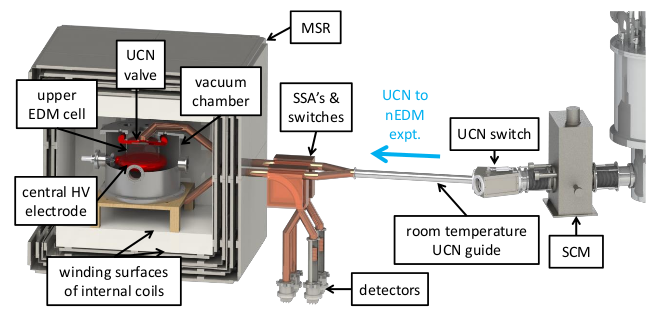
\includegraphics[width=1.0\textwidth]{UCNdelivery.png}
%  \caption{UCN delivery and the nEDM experiment. UCN exit the source
%    by passing through the SCM spin polarizer and UCN switch and
%    detector system, where they then enter the proposed Phase 2 nEDM
%    experiment. UCN are loaded into the measurement cells within a
%    MSR/coil system. At the end of the measurement cycle, UCN are
%    counted by simultaneous spin analyzers (SSA’s) including
%    detectors. An ambient magnetic compensation system and thermally
%    controlled room which will surround the nEDM apparatus~(not
%    shown). For scale, the innermost layer of the MSR is a 1.8~m
%    side-length cube.}
%  \label{fig:UCNdelivery}
%\end{figure}



%\subsection{DAQ?}
%\begin{description}
%\item{An introduction about the long term nEDM effort at TRIUMF, what
% the plan is, when it will start (roughly). I guess I can probably
% get this information from some proposals. I am not sure how much
% detail should go here.}
  
%\item{How the EDM experiment is actually done, talk about different
%  components of the system. Here is where I talk about the Ramsey
%  cycle ...}
  
%\item{nEDM measurement systematic effects: This is where I talk about
%  the GPE and ... . Basically here is to kind of motivate that we need
%  to have stable magnetic fields and we need lots of neutrons.}
  
%\item{Introduction to the magnetic stability requirements at
%  TRIUMF. What I mean is that there is 400 $\mu$T background field at
%  TRIUMF. Hopefully we have a field map of the area soon(?).}
  
%\item{From ouside in: Magnetically shielded room, what is the status
%  of that, are we going to have it? when? How good is it going to be
%  compared to the other ones worldwide? Why is it designed that way?
%  What is the design? Drawings of it. General question: Some of these
%  are about things that will happen in the future and I have not
%  worked on them. Should they even go to my thesis? I feel I have to
%  say a little about this since my thesis is nEDM related and it is
%  part of it.}
  
%\item{Passive shieldings: Again same questions as above, motivate for
%  the next chapter}

  
%\item{Say what will be discussed in the two coming chapters}
  
%\item{what else?}
%\end{description}